%----------createParameter----------------------------------------
\op
{createParameter}
{creates a new parameter}
{createParameter(Operation selectedEObject, String nameValue)}
{The operation providing the container for the newly created parameter.}
{
\begin{itemize}
 \item nameValue/newName: The name of the newly created parameter
 \item idValue/newID: The id of the newly created parameter
\end{itemize}
}
{There is no parameter in the same context whose name equals the parameter-value
of 'newName' (see
\ref{subsec:checkOtherNames})} 
{Only the name and the id will be set via input data. kind will be set
with a default value as defined with the diagram editor in the image below.}
\begin{figure}[H]
  \centering
  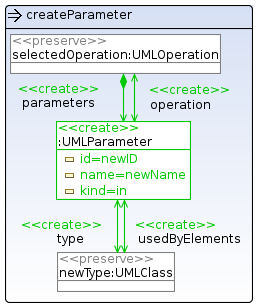
\includegraphics[width=0.4\textwidth]{pics/createParameter.png}
  \caption{createParameter}
  \label{createParameter}
\end{figure}
%----------deleteParameter----------------------------------------
\op
{deleteParameter}
{Deletes an parameter}
{deleteParameter(Parameter selectedEObject)}
{The parameter which should be deleted}
{-}
{-}
{For a better readability this is a simplified version of the
'deleteParameter'-transformation and will only cover cases where the
parameter has no references to other elements. Such a
complex transformation rule exits but won't be listed here.}
\begin{figure}[H]
  \centering
  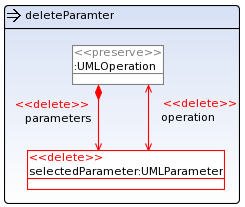
\includegraphics[width=0.4\textwidth]{pics/deleteParameter_emptyAndUnreferenced.png}
  \caption{createParameter}
  \label{createParameter}
\end{figure}
%----------editParameterName----------------------------------------
\op
{editParameterName}
{edits the name of an parameter}
{editParameterName(Parameter selectedEObject, String nameValue)}
{The parameter whose name should be renamed.}
{
\begin{itemize}
 \item nameValue/newName: The new name
\end{itemize}
}
{There is no parameter in the same operation whose name equals the parameter-value of
'newName' (see
\ref{subsec:checkOtherNames})}
{The \textless\textless create\textgreater\textgreater  -symbol in the image
means that even if the attribute exists its value will be overwritten.
'someName' is the placeholder for the input name.}
\begin{figure}[H]
  \centering
  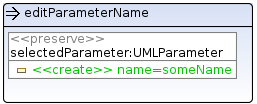
\includegraphics[width=0.4\textwidth]{pics/editParameterName.png}
  \caption{editParameterName}
  \label{editParameterName}
\end{figure}
%----------editParameterKind----------------------------------------
\op
{editParameterKind}
{edits the kind-value (in;out) of an parameter}
{editParameterKind(Parameter selectedEObject, Kind newParameterKindValue)}
{The parameter whose kind-value should be edited.}
{
\begin{itemize}
 \item newParameterKindValue/parameterKind: The new kind-value
\end{itemize}
}
{-}
{The \textless\textless create\textgreater\textgreater  -symbol in the image
means that even if the attribute exists its value will be overwritten.
'parameterKind' is the placeholder for the input parameterKind.}
\begin{figure}[H]
  \centering
  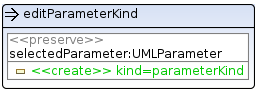
\includegraphics[width=0.4\textwidth]{pics/editParameterKind.png}
  \caption{editParameterKind}
  \label{editParameterKind}
\end{figure}
%----------editParameterTypeFromClassToClass----------------------------------------
\op
{editParameterTypeFromClassToClass}
{edits the type of an parameter from a class to another}
{editParameterTypeFromClassToClass(Parameter selectedEObject, Class typeValue)}
{The parameter whose type should be edited.}
{
\begin{itemize}
 \item typeValue/newType: The new type
\end{itemize}
}
{-}
{Only references will change.}
\begin{figure}[H]
  \centering
  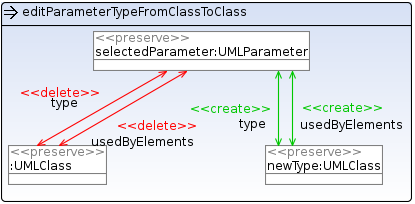
\includegraphics[width=0.65\textwidth]{pics/editParameterTypeFromClassToClass.png}
  \caption{editParameterTypeFromClassToClass}
  \label{editParameterTypeFromClassToClass}
\end{figure}
%----------editParameterTypeFromClassToPrimitive----------------------------------------
\op
{editParameterTypeFromClassToPrimitive}
{edits the type of an parameter from a class to a primitiveType}
{editParameterTypeFromClassToPrimitive(Parameter selectedEObject, PrimitiveType typeValue)}
{The parameter whose type should be edited.}
{
\begin{itemize}
 \item typeValue/newType: The new type
\end{itemize}
}
{-}
{-}
{Only references will change.}
\begin{figure}[H]
  \centering
  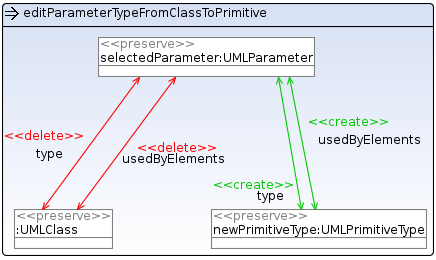
\includegraphics[width=0.65\textwidth]{pics/editParameterTypeFromClassToPrimitive.png}
  \caption{editParameterTypeFromClassToPrimitive}
  \label{editParameterTypeFromClassToPrimitive}
\end{figure}
%----------editParameterTypeFromPrimitiveToClass----------------------------------------
\op
{editParameterTypeFromPrimitiveToClass}
{edits the type of an parameter from a primitiveType to a class}
{editParameterTypeFromPrimitiveToClass(Parameter selectedEObject, Class typeValue)}
{The parameter whose type should be edited.}
{
\begin{itemize}
 \item typeValue/newType: The new type
\end{itemize}
}
{-}
{-}
{Only references will change.}
\begin{figure}[H]
  \centering
  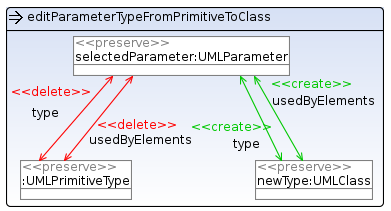
\includegraphics[width=0.60\textwidth]{pics/editParameterTypeFromPrimitiveToClass.png}
  \caption{editParameterTypeFromPrimitiveToClass}
  \label{editParameterTypeFromPrimitiveToClass}
\end{figure}
%----------editParameterTypeFromPrimitiveToPrimitive----------------------------------------
\op
{editParameterTypeFromPrimitiveToPrimitive}
{edits the type of an parameter from a primitiveType to a primitiveType}
{editParameterTypeFromPrimitiveToPrimitive(Parameter selectedEObject, PrimitiveType typeValue)}
{The parameter whose type should be edited.}
{
\begin{itemize}
 \item typeValue/newType: The new type
\end{itemize}
}
{-}
{-}
{Only references will change.}
\begin{figure}[H]
  \centering
  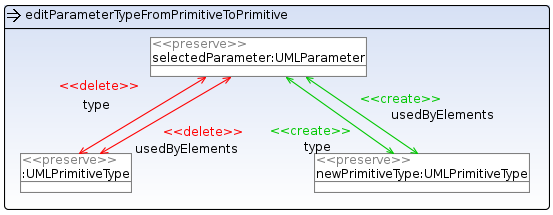
\includegraphics[width=0.8\textwidth]{pics/editParameterTypeFromPrimitiveToPrimitive.png}
  \caption{editParameterTypeFromPrimitiveToPrimitive}
  \label{editParameterTypeFromPrimitiveToPrimitive}
\end{figure}
%----------moveParameter----------------------------------------
\op
{moveParameter}
{moves an parameter from a operation to another operation}
{moveParameter(Parameter selectedEObject, Operation tgt)}
{The parameter which should be moved.}
{
\begin{itemize}
 \item tgt/tgt[moveParameter]: the target operation
\end{itemize}
}
{There is no parameter with the same name in the target context (see
\ref{subsec:checkOtherNames})}
{Only references will change.}
\begin{figure}[H]
  \centering
  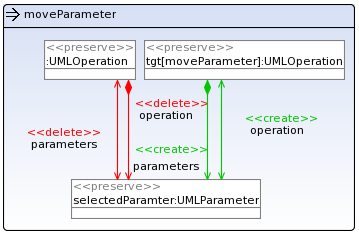
\includegraphics[width=0.55\textwidth]{pics/moveParameter.png}
  \caption{moveParameter}
  \label{moveParameter}
\end{figure}